\newcommand*{\ls}{Linear Scaling}%
\subsection{\ls{}}\label{sub:ls}
\forceendwrapfig{}
Ο \ls{} (LS) είναι ένας απλός αλγόριθμος για matching μελωδίας.
Προσπαθεί να μεγαλώσει ή να μικρύνει το pitch γραμμικά έτσι ώστε να ταιριάξει
με το υποψήφιο MIDI τραγούδι στο database. Από μόνος του έχει πολλά
μειονεκτήματα. Για παράδειγμα, τοπικές διαφορές μπορεί να επηρεάσουν πολύ την
γενική εικόνα.

\begin{wrapfigure}{r}{0.5\textwidth}
        \centering
        \vspace{-20pt}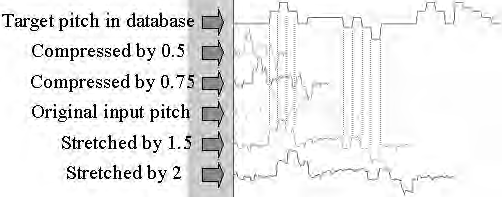
\includegraphics[width=\linewidth]{linear-scaling}
        \vspace{-20pt}\caption{Παράδειγμα \ls{} από \protect\cite{jang2005continuous}}
        \label{fig:linear-scaling}
\end{wrapfigure}

Ωστόσο, βρίσκει σημαντική πρακτική αξία σε συστήματα QbSH σε συνδυασμό με άλλες
τεχνικές. Αναφορικά, χρησιμοποιήθηκε σε συνδυασμό με Hidden Markov Models το
2005 στο \cite{jang2005continuous} και χρησιμοποιείται στον Recursive Alignment
αλγόριθμο στο \cite{wu2006top}.
\undef{\ls}
